\makeatletter\def\input@path{{../template/vsp-beamer}{../template/minimus}}\makeatother

\documentclass[red,tutorial,sectionpages,shtu]{vsp-beamer}
\graphicspath{{image/}{../template/vsp-beamer/assets/}}

\usepackage{minimus-section}
\usepackage{minimus-text}
\usepackage{minimus-math}
\usepackage{minimus-float}
\usepackage{minimus-code}
\usepackage{minimus-colorbox}
\usepackage{minimus-reference}

\title{CS100 Introduction}
\subtitle{从写代码到解决问题}
\VSPsetspeaker{CS100 Teaching Assistants}{ShanghaiTech University}
\VSPsetupfootline{CS100 Introduction}{Fall 2026}{CS100 TAs}

\begin{document}
\VSPtitleframe
\section{首先，致敬伟人GKxx}

\begin{frame}{革命尚未成功，同志仍须努力}
    \begin{center}
        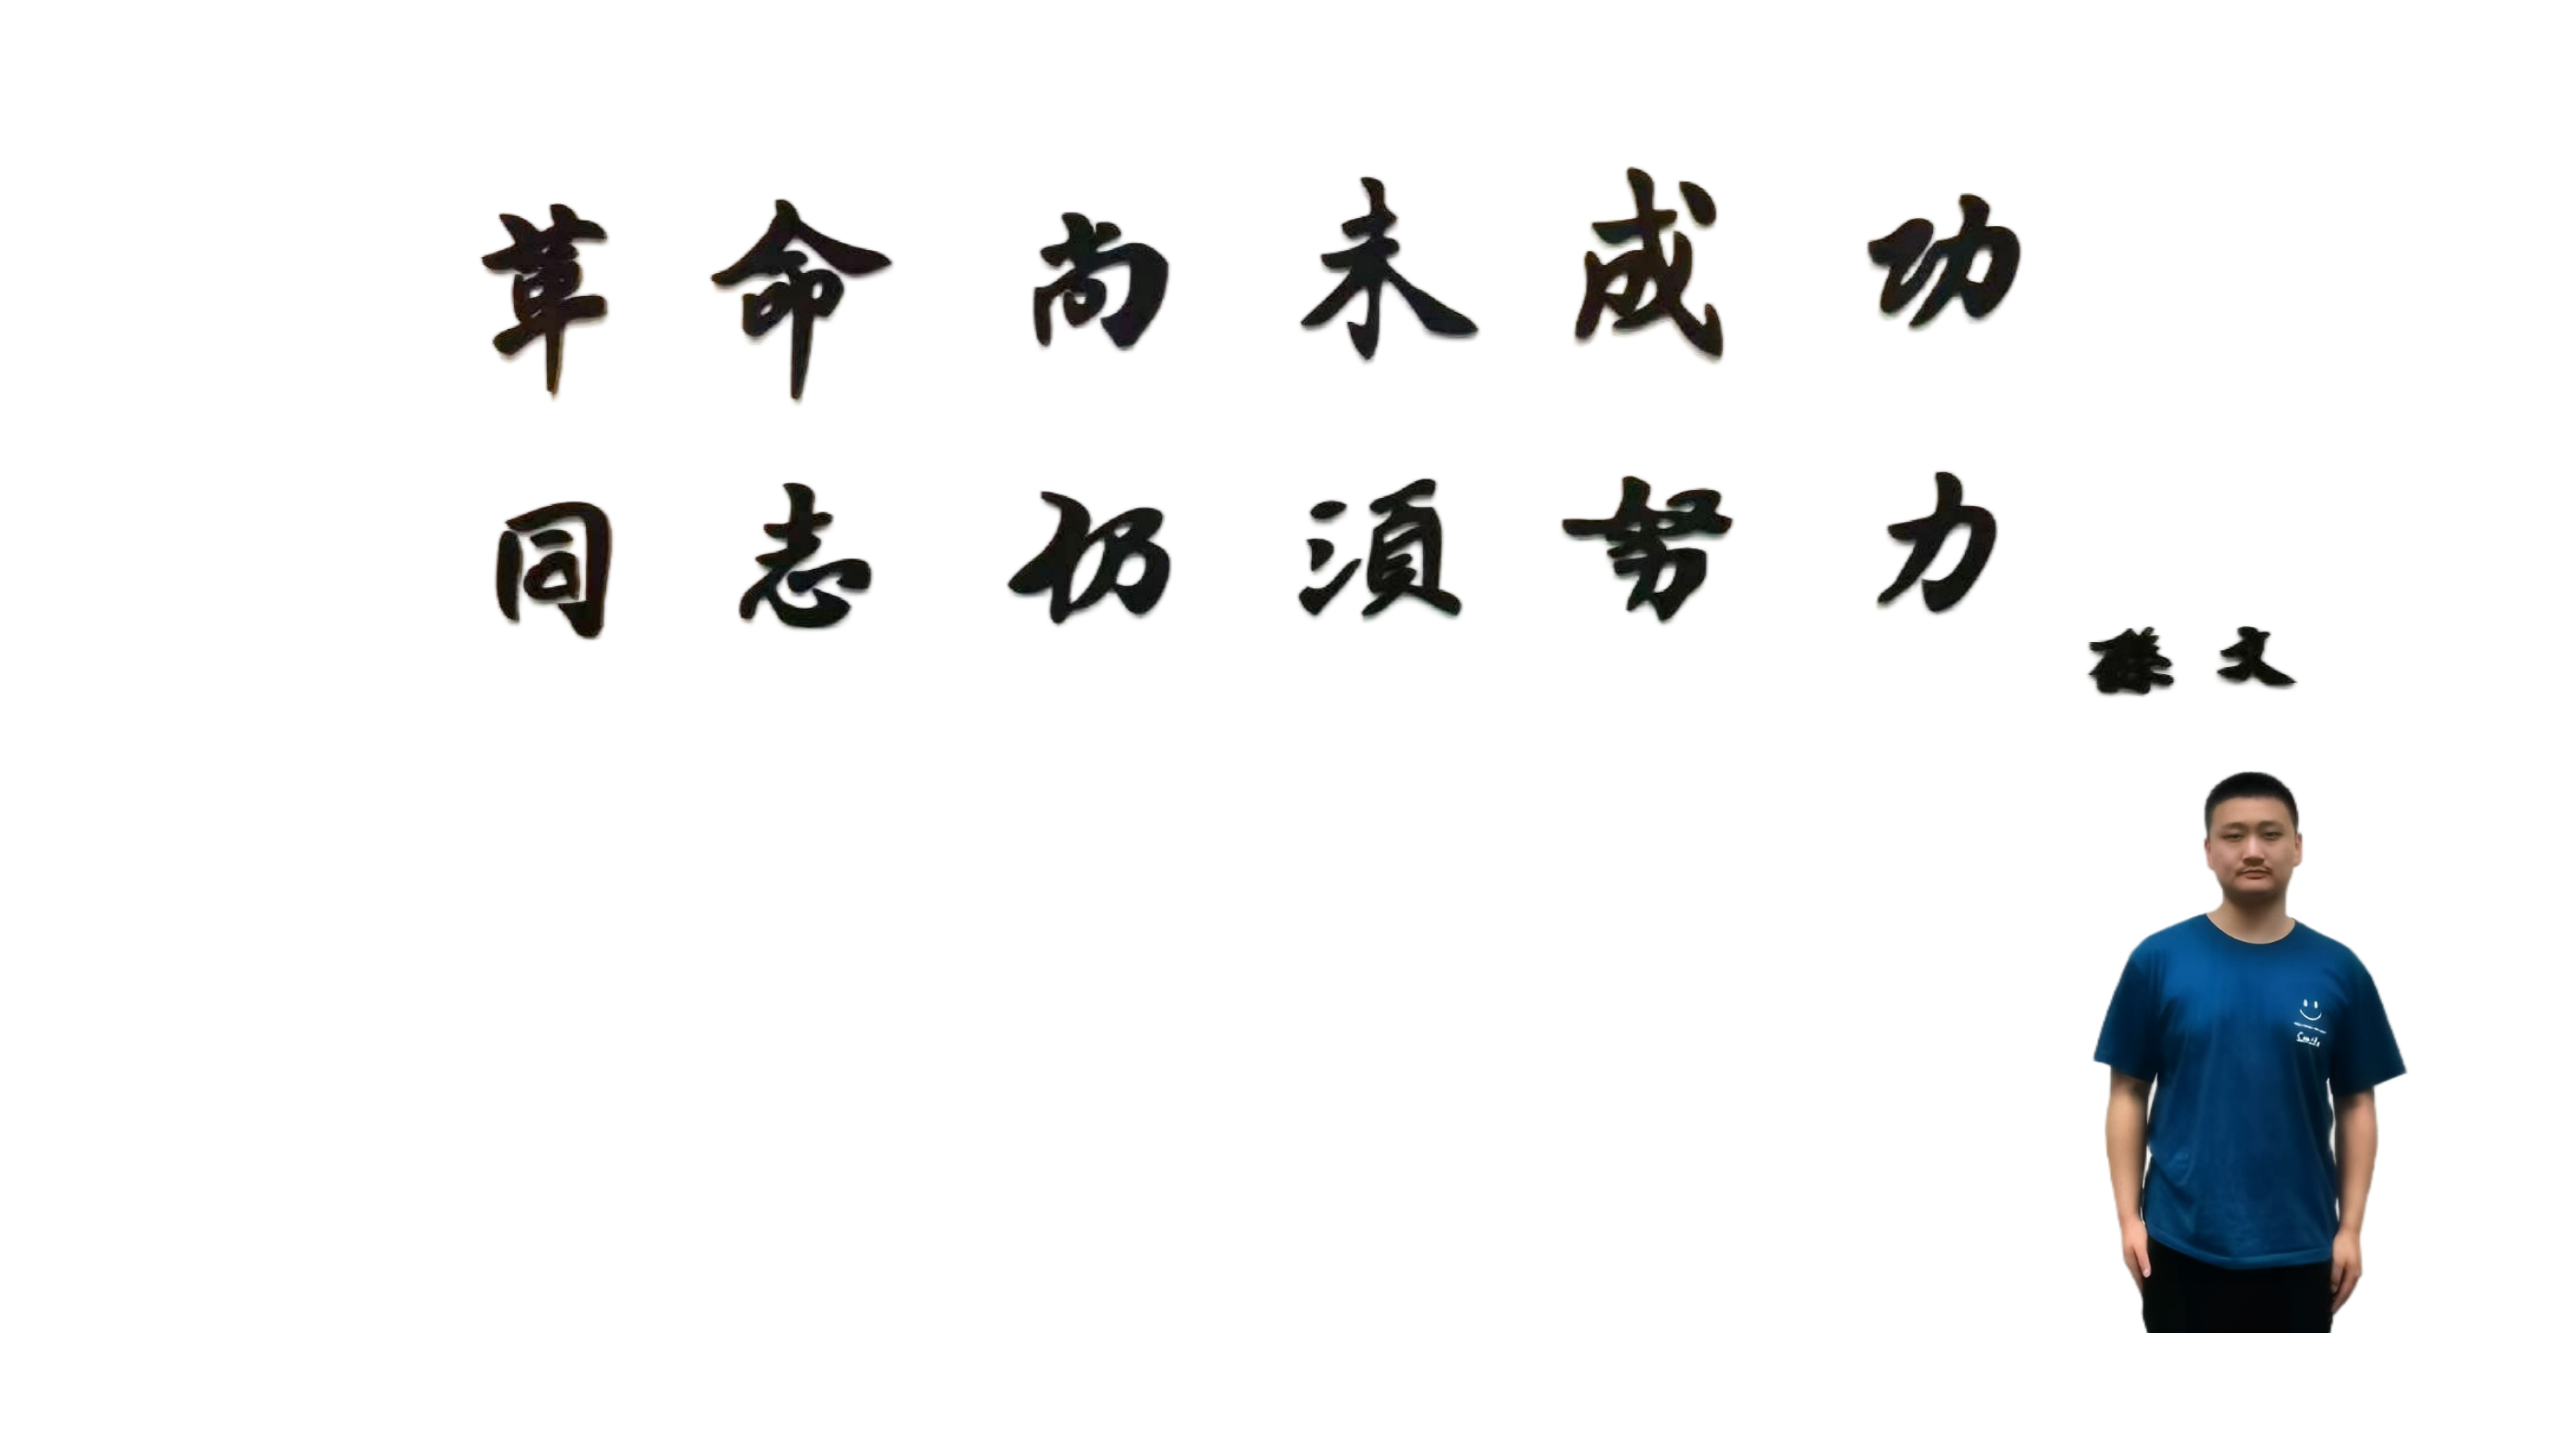
\includegraphics[width=\linewidth,height=0.72\textheight,keepaspectratio]{gkxx.png}
    \end{center}
\end{frame}

\begin{frame}{GKxx：现代CS100的重要建设者}
    GKxx是上海科技大学2020级计算机科学与技术专业学生，曾多次担任CS100的TA。

    \begin{itemize}
        \item 深度参与课程建设，推动课件内容与教学方式的改良。
        \item 改进课程考核，为我们今天的CS100打下了重要基础。
        \item 如今已经“飞升”国科大／中国科学院软件研究所。
    \end{itemize}

    \begin{vspquote}{致敬，也接力}
        今天的课程建立在前人的投入之上。把课讲清楚，把工具做好，把这份认真传下去。
    \end{vspquote}

    Bilibili：\textbf{GKxxISCAS}\qquad
    GitHub：\href{https://github.com/GKxxUCAS}{\textbf{GKxxUCAS}}
\end{frame}

\section{认识你的TA}

\begin{frame}{HeadTA：李超凡}
    \begin{columns}[c]
        \begin{column}{0.30\textwidth}
            
\includegraphics[width=\linewidth]{LCF.jpg}
        \end{column}
        \begin{column}{0.66\textwidth}
            \small
            \alert{2021届本科生／2025届博士研究生}\par
            娄鑫课题组招新大使\quad CET6备战中
            \medskip

            \alert{助教经历}
            \begin{itemize}
                \item 2022 Fall至今：信导助教
                \item 2024--2026 Fall：CS100 HeadTA
                \item 2026 Spring：CS110优秀TA
            \end{itemize}
            \medskip
            \alert{竞赛与带队}
            \begin{itemize}
                \item 2023届iGEM全球前十、金奖
                \item 2023年电赛二等奖
                \item 2025年金牌电赛教练
            \end{itemize}
        \end{column}
    \end{columns}
\end{frame}

\begin{frame}{TA：李宇轩}
    \begin{columns}[c]
        \begin{column}{0.30\textwidth}
            
\includegraphics[width=\linewidth]{LYX.png}
        \end{column}
        \begin{column}{0.66\textwidth}
            \small
            \alert{2021届上海大学微电子专业优秀毕业生}\par
            2025届娄组工程博士
            \medskip

            \alert{助教经历}
            \begin{itemize}
                \item 2025 Fall、2026 Spring：信导助教
                \item 2026 Spring：CS110计算机体系结构助教
            \end{itemize}
            \medskip
            {\color{black}Windows与Verilog的{\bfseries 掘墓人}\par
            \LaTeX{}古法TikZ的{\bfseries 非遗传承者}\par
            Spinal、Linux、\LaTeX{}、Vim宣传大使\par}
        \end{column}
    \end{columns}
\end{frame}

% JY与WSH的个人介绍暂留空，等待补充。
\begin{frame}{TA：JY}
\end{frame}

\begin{frame}{TA：WSH}
\end{frame}

\begin{frame}{怎样让TA更快帮到你？}
    “我的代码不行”很难定位；一个\alert{可以复现的问题}更容易得到有效帮助。
    \begin{enumerate}
        \item 我想做什么？题目要求、输入与预期输出是什么？
        \item 实际发生了什么？提供最小代码、实际输出和完整报错。
        \item 在什么环境发生？系统、编译器版本、编译与运行命令。
        \item 我已经尝试过什么？哪些修改改变了现象？
    \end{enumerate}
    \alert{优先提供可复制的代码与文字}，让别人能在自己的环境中重现问题。
\end{frame}

\section{我们为什么学习编程？}

\begin{frame}{编程要解决什么问题？}
    编程是把一个需求，变成计算机可以\alert{重复、准确地执行的过程}。
    \begin{itemize}
        \item 自动化：把一千份文件按规则整理，而不是手动点一千次。
        \item 数据处理：从一批观测中提取信息，而不是只盯着原始数字。
        \item 建模与计算：把现实问题抽象成数据、约束与算法。
        \item 构建系统：让多个功能组合起来，持续、可靠地工作。
    \end{itemize}
    语言是表达方案的工具。真正需要你决定的是：\alert{做什么、怎样做、怎样证明做对了}。
\end{frame}

\begin{frame}{从一句需求，到一个明确的问题}
    需求：“帮我算一下全班的平均成绩。”
    \begin{enumerate}
        \item \alert{明确输入}：成绩从哪里来？一共有多少人？是否合法？
        \item \alert{约定规则}：缺考如何处理？空名单怎么办？保留几位小数？
        \item \alert{设计步骤}：读取数据，检查约束，累加求和，计算并输出。
        \item \alert{验证结果}：用能手算的小例子和边界情况检查程序。
    \end{enumerate}
    计算机不会替你补全含糊的需求，AI生成代码也不能替你决定这些规则。
\end{frame}

\begin{frame}{为什么还要学C语言？}
    C让许多被高级抽象隐藏的细节，成为你必须理解的对象。
    \begin{itemize}
        \item \alert{数据表示}：类型、取值范围与精度，都会影响计算结果。
        \item \alert{内存模型}：数组、地址、指针、对象的生存期。
        \item \alert{程序执行}：源文件怎样经过编译与链接，变成可执行程序。
        \item \alert{资源与代价}：一次复制、一次分配、一个循环意味着什么。
    \end{itemize}
    学C帮助我们建立程序如何运行的基本模型，为后续系统课程打基础。
\end{frame}

\begin{frame}{C和Python：不同的抽象层次}
    \small
    \renewcommand{\arraystretch}{1.4}
    \begin{tabular}{p{0.15\linewidth}p{0.36\linewidth}p{0.36\linewidth}}
        \alert{维度} & \alert{C} & \alert{Python} \\
        类型 & 变量有声明的类型 & 对象有类型，名字可绑定不同对象 \\
        整数 & 常用整数类型有固定取值范围 & 内置整数支持任意精度，受可用内存限制 \\
        内存 & 直接使用地址；动态内存需显式管理 & 通常由运行时管理对象内存 \\
        容器 & 数组长度与索引范围需自行留意 & 内置列表、字典等高级容器 \\
        执行 & 通常先编译、链接，再运行 & 通常由解释器运行；也可能涉及字节码 \\
    \end{tabular}
    \medskip

    两种语言都可以表达算法；它们让你直接控制的细节、承担的责任不同。
\end{frame}

\begin{frame}{一个比喻：全能翻译官与译好的书}
    \begin{columns}[T]
        \begin{column}{0.47\textwidth}
            \alert{Python：带着一位全能翻译官}
            \begin{itemize}
                \item 这位“翻译官”就是\alert{解释器}，在程序运行时帮助执行代码。
                \item 去中国讲中文，去法国讲法语：各个平台有适配自己的解释器。
                \item 同一份代码通常可以跨平台运行，前提是解释器和依赖兼容。
            \end{itemize}
        \end{column}
        \begin{column}{0.47\textwidth}
            \alert{C：一本已经译成中文的书}
            \begin{itemize}
                \item \alert{编译器}提前完成翻译，得到目标平台的可执行程序。
                \item 中国读者直接读，不必现场翻译，通常执行效率较高。
                \item 拿给不懂中文的法国读者就看不懂：换平台往往需要重新编译。
            \end{itemize}
        \end{column}
    \end{columns}
    \medskip
    这里的“中文书”指\alert{编译后的程序}。C源代码仍可移植；能否直接运行，取决于操作系统、处理器架构等条件。
\end{frame}

\begin{frame}{同一道算术题，为什么答案不同？}
    \begin{columns}[T]
        \begin{column}{0.47\textwidth}
            \alert{C：先看操作数的类型}
            \begin{Code}*{c}
                \lstinputlisting{code/division.c.txt}
            \end{Code}
            两个整数相除，结果仍是整数；再赋给\code{double}也不会恢复小数部分。
        \end{column}
        \begin{column}{0.47\textwidth}
            \alert{Python 3：区分两种除法}
            \begin{Code}*{python}
                \lstinputlisting{code/division.py}
            \end{Code}
            \code{/}表示真除法，\code{//}表示向下取整的除法。
        \end{column}
    \end{columns}
    \medskip
    学习差异，是为了理解代码的含义。比如负数参与时，C的整数除法向零截断，Python的\code{//}向下取整。
\end{frame}

\begin{frame}{我们不做“语言律师”}
    我们不把背诵冷僻规则、猜测刁钻表达式的输出当作学习目标。

    但你需要理解与正确性直接相关的规则：
    \begin{itemize}
        \item 类型转换和整数除法，是否改变了你想计算的东西？
        \item 数组索引是否越界？变量是否已经初始化？
        \item 一个地址指向的对象，是否仍然存在？
        \item 程序是否依赖未定义行为，导致结果无法保证？
    \end{itemize}
    \alert{写清晰、可解释的代码；遇到不确定的规则，查文档、做验证。}
\end{frame}

\begin{frame}{AI时代，哪些能力更重要？}
    AI能帮助解释报错、生成代码、提出思路，但你仍然需要：
    \begin{enumerate}
        \item \alert{定义问题}：把输入、输出、约束与例外说清楚。
        \item \alert{审查方案}：理解算法、数据结构和复杂度是否合适。
        \item \alert{验证行为}：设计测试，用证据判断结果是否正确。
        \item \alert{承担责任}：能解释、修改和维护最终提交的代码。
    \end{enumerate}
    \begin{vspquote}{一个简单的自检}
        如果这段代码明天出错，你能从哪里开始查？
    \end{vspquote}
\end{frame}

\begin{frame}{把AI放进有反馈的学习过程}
    \begin{enumerate}
        \item 先自己写出问题描述、思路和几个预期结果。
        \item 请求提示、解释或方案比较，并指出自己卡在哪里。
        \item 逐段读懂代码，在统一环境中编译并检查诊断信息。
        \item 用正常输入、边界输入与反例验证，发现问题后再修改。
    \end{enumerate}
    \alert{编译成功不等于逻辑正确，几个样例通过也不等于程序正确。}

    作业与考试能否使用AI、如何说明使用情况，以当次课程要求为准。
\end{frame}

\begin{frame}{为什么CS100要规范开发方式？}
    “在我电脑上能跑”，还不足以让别人复现你的结果。
    \begin{itemize}
        \item \alert{统一编译环境}：减少系统、语言标准和编译选项造成的差异。
        \item \alert{统一代码习惯}：让同学、TA和未来的自己都能读懂代码。
        \item \alert{使用版本管理}：知道改了什么，保留可运行的版本。
        \item \alert{保留验证过程}：提交的结果可以被重新构建和检查。
    \end{itemize}
    这些习惯从第一个小程序就开始建立，不必等到项目变大。
\end{frame}

\begin{frame}{编译环境：让构建过程可复现}
    本课程统一使用\alert{C17和C++17}；习题课沿用r0的Ubuntu／WSL与GCC路线。
    \begin{Code}*{bash}
        \lstinputlisting{code/build.sh}
    \end{Code}
    \begin{itemize}
        \item 显式指定语言标准，避免依赖编译器的默认设置。
        \item 开启常用警告，逐条理解并修复，不把警告当作背景噪声。
        \item 记录系统、编译器版本和命令；编辑器可以不同，构建过程要清楚。
    \end{itemize}
    \small C源文件使用gcc，C++源文件使用g++。编译器具体版本及其他评测参数，以课程公告为准。
\end{frame}

\begin{frame}{代码习惯：写给人读，也交给机器执行}
    \begin{itemize}
        \item \alert{命名表达含义}：用\code{student_count}表达人数，避免一串无意义缩写。
        \item \alert{格式保持一致}：统一缩进、括号和空格，让结构一眼可见。
        \item \alert{拆分职责}：一个函数完成一件清楚的事，减少重复与隐含依赖。
        \item \alert{注释解释原因}：说明约束、假设和设计选择，不逐句翻译代码。
        \item \alert{尊重题目接口}：严格遵守输入输出格式，不夹带调试信息。
    \end{itemize}
    代码越容易读懂，就越容易发现错误、验证行为和继续修改。
\end{frame}

\begin{frame}{版本管理：不要再用“最终版2”}
    Git把每次有意义的修改保存成一个可以回看的版本。
    \begin{Code}*{bash}
        \lstinputlisting{code/version-control.sh}
    \end{Code}
    \begin{itemize}
        \item 一次提交围绕一件事，提交信息说明这次改变的含义。
        \item 提交源码与必要配置，用\code{.gitignore}排除生成文件。
        \item Git可以完全在本地使用；如需远端备份，课程作业应遵守公开范围要求。
    \end{itemize}
\end{frame}

\begin{frame}{一次小修改，也值得走完这个循环}
    \begin{center}
        {\Large 明确问题\ $\rightarrow$\ 编写代码\ $\rightarrow$\ 编译检查}\par
        \medskip
        {\Large 测试验证\ $\rightarrow$\ 检查差异\ $\rightarrow$\ 提交版本}
    \end{center}
    \begin{itemize}
        \item \alert{正常情况}：输入几条普通成绩，与手算结果对照。
        \item \alert{边界情况}：只有一条记录、零分、满分，是否符合约定？
        \item \alert{特殊情况}：空输入与不合法数据，按题目约定处理。
        \item \alert{回归检查}：修好一个问题后，原来正确的情况是否仍然正确？
    \end{itemize}
    每次只改清楚的一件事，你会更容易知道：这次为什么变好了，哪里又出了问题。
\end{frame}

\begin{frame}{我们希望你带走什么？}
    \begin{enumerate}
        \item 能把模糊需求转化为明确的问题与可执行的步骤。
        \item 能解释程序的行为，理解数据、内存与计算的基本模型。
        \item 能使用工具定位问题，并用测试验证自己的判断。
        \item 能留下清楚的代码、可复现的环境与可追溯的修改记录。
    \end{enumerate}
    \begin{vspquote}{从CS100开始}
        让代码值得信任，让自己有能力判断它为什么值得信任。
    \end{vspquote}
\end{frame}

\VSPendframe{}
\end{document}
